\documentclass[11pt,letterpaper]{article}

\usepackage[utf8]{inputenc}
\usepackage[T1]{fontenc}
\usepackage[spanish,es-nodecimaldot]{babel}
\usepackage{amsmath,amssymb,amsfonts}
\usepackage{booktabs}
\usepackage{array}
\usepackage{graphicx}
\usepackage{float}
\usepackage{geometry}
\usepackage{xcolor}
\usepackage{hyperref}
\usepackage{caption}
\usepackage{subcaption}

\geometry{margin=2.35cm}
\graphicspath{{outputs_sbm_sw/}}

\hypersetup{
    colorlinks=true,
    linkcolor=blue!45!black,
    urlcolor=blue!45!black,
    citecolor=blue!45!black
}

\title{Caso de estudio: DC-SBM en la red de personajes de Star Wars II}
\author{LDS1121 - Redes complejas}
\date{}

\newcommand{\Gmini}{G_{\mathrm{mini}}}
\newcommand{\Omhat}{\hat\Omega}

\begin{document}

\maketitle

\begin{abstract}
Este reporte interpreta el ajuste de un modelo de bloques estocásticos corregido por grado a la red de personajes de \emph{Star Wars II: Attack of the Clones}, correspondiente al archivo \texttt{data/dataverse/gexf/774.gexf}. La notación sigue el apunte \emph{Métodos basados en inferencia estadística}: los grupos se indexan como $1,\ldots,q$, la asignación latente es $g=(g_1,\ldots,g_n)$, los parámetros de grado esperado son $c_i$ y la matriz de intensidades comunitarias es $\Omega=(\omega_{rs})$. El criterio penalizado selecciona $q=6$ para la red completa y $q=5$ para la minired. El resultado muestra una mezcla de subtramas densas y personajes puente: algunos bloques son asortativos, mientras otros existen porque conectan intensamente partes distintas de la narración.
\end{abstract}

\section{Datos y pregunta}

La red se lee desde
\[
\texttt{data/dataverse/gexf/774.gexf}.
\]
El grafo es no dirigido, tiene $47$ personajes y $148$ aristas. La minired $\Gmini$ se construyó conservando personajes de grado al menos $3$:
\[
V_{\mathrm{mini}}=\{i\in V:\; k_i\ge 3\},
\qquad
\Gmini=G[V_{\mathrm{mini}}],
\]
lo que deja $34$ personajes y $128$ aristas.

La pregunta central es:

\begin{quote}
¿La red de personajes se organiza como comunidades densas, como roles narrativos que conectan subtramas, o como una mezcla de ambas cosas?
\end{quote}

Esta distinción importa porque una red narrativa no necesariamente se comporta como una red social con grupos cerrados. Personajes como Padmé, Obi-Wan y Anakin tienen grado alto porque cruzan escenas y subtramas. El modelo corregido por grado separa esa centralidad individual de la estructura comunitaria.

\section{Modelo y notación}

Sea $A$ la matriz de adyacencia no dirigida. El grado observado del personaje $i$ es
\[
k_i=\sum_j A_{ij},
\qquad
2m=\sum_i k_i.
\]
En el modelo de bloques estocásticos corregido por grado, cada nodo pertenece a un grupo
\[
g_i\in\{1,\ldots,q\}.
\]
La probabilidad, o intensidad Poisson, de una arista entre $i$ y $j$ es proporcional a
\[
\omega_{g_i g_j}\frac{c_i c_j}{2m}.
\]
Aquí $c_i$ captura la propensión individual del personaje $i$ a conectarse, mientras que $\omega_{rs}$ mide la intensidad de interacción entre los grupos $r$ y $s$.

Para una partición fija $g$, definimos
\[
\kappa_r=\sum_i \delta_{g_i r}c_i,
\qquad
m_{rs}=\sum_{ij}\delta_{g_i r}\delta_{g_j s}A_{ij}.
\]
Al maximizar la verosimilitud respecto a los parámetros continuos, se obtiene
\[
\hat c_i=k_i,
\qquad
\hat\omega_{rs}=\frac{2m\,m_{rs}}{\kappa_r\kappa_s}.
\]
Luego la log-verosimilitud perfilada es
\[
L(g)=
\frac{1}{2}\sum_{r,s}
m_{rs}\log\left(\frac{m_{rs}}{\kappa_r\kappa_s}\right)
+\text{constantes}.
\]
Por tanto, para cada $q$ buscamos
\[
\hat g_q=\arg\max_{g:V\to\{1,\ldots,q\}}L(g).
\]

\subsection{Por qué la corrección por grado cambia la interpretación}

La fórmula
\[
\hat\omega_{rs}=\frac{2m\,m_{rs}}{\kappa_r\kappa_s}
\]
no solo cuenta aristas. Si dos grupos contienen personajes muy centrales, entonces $\kappa_r\kappa_s$ será grande y se esperaría cierta cantidad de aristas aun sin estructura especial. Por eso $\hat\omega_{rs}$ mide exceso de interacción entre grupos después de corregir por grado.

Esto es crucial en Star Wars II. Padmé, Obi-Wan y Anakin tienen grados $30$, $29$ y $24$ en la red completa. Sin corrección por grado, podrían dominar cualquier partición. Con DC-SBM, primero se fija $\hat c_i=k_i$ y luego se pregunta dónde caen las aristas \emph{más de lo esperado} dado ese grado.

\section{Selección del número de grupos}

Se evaluaron varios valores de $q$ y se usó el criterio penalizado
\[
\operatorname{BIC}_{\mathrm{like}}(q)
=-2\hat L_q+p_q\log(2m),
\qquad
p_q\approx \frac{q(q+1)}{2}-q.
\]

\begin{table}[H]
\centering
\caption{Barrido de $q$ para la red completa y la minired. Menor BIC-like es mejor.}
\resizebox{\textwidth}{!}{%
\begin{tabular}{llrrr}
\toprule
Red & $q$ & $L$ perfilada & BIC-like & Modularidad diagnóstica\\
\midrule
$G$ & 2 & -1386.927 & 2779.544 & 0.248\\
$G$ & 3 & -1361.020 & 2739.110 & 0.125\\
$G$ & 4 & -1338.741 & 2711.623 & 0.183\\
$G$ & 5 & -1320.584 & 2698.073 & 0.212\\
$G$ & 6 & -1305.318 & \textbf{2695.992} & 0.146\\
$G$ & 7 & -1293.018 & 2705.534 & 0.117\\
$G$ & 8 & -1276.739 & 2712.808 & 0.145\\
\midrule
$\Gmini$ & 2 & -1228.973 & 2463.491 & 0.251\\
$\Gmini$ & 3 & -1206.781 & 2430.197 & 0.114\\
$\Gmini$ & 4 & -1187.248 & 2407.767 & 0.175\\
$\Gmini$ & 5 & -1172.257 & \textbf{2399.965} & 0.140\\
$\Gmini$ & 6 & -1159.504 & 2402.186 & 0.165\\
$\Gmini$ & 7 & -1149.048 & 2414.545 & 0.167\\
\bottomrule
\end{tabular}
}
\end{table}

La red completa selecciona $q=6$ y la minired selecciona $q=5$. La modularidad no es máxima en esos puntos, pero eso no invalida el resultado. La modularidad favorece comunidades asortativas; el DC-SBM también puede detectar roles y bloques puente. En una historia con subtramas cruzadas, esto es precisamente lo que buscamos.

\begin{figure}[H]
\centering
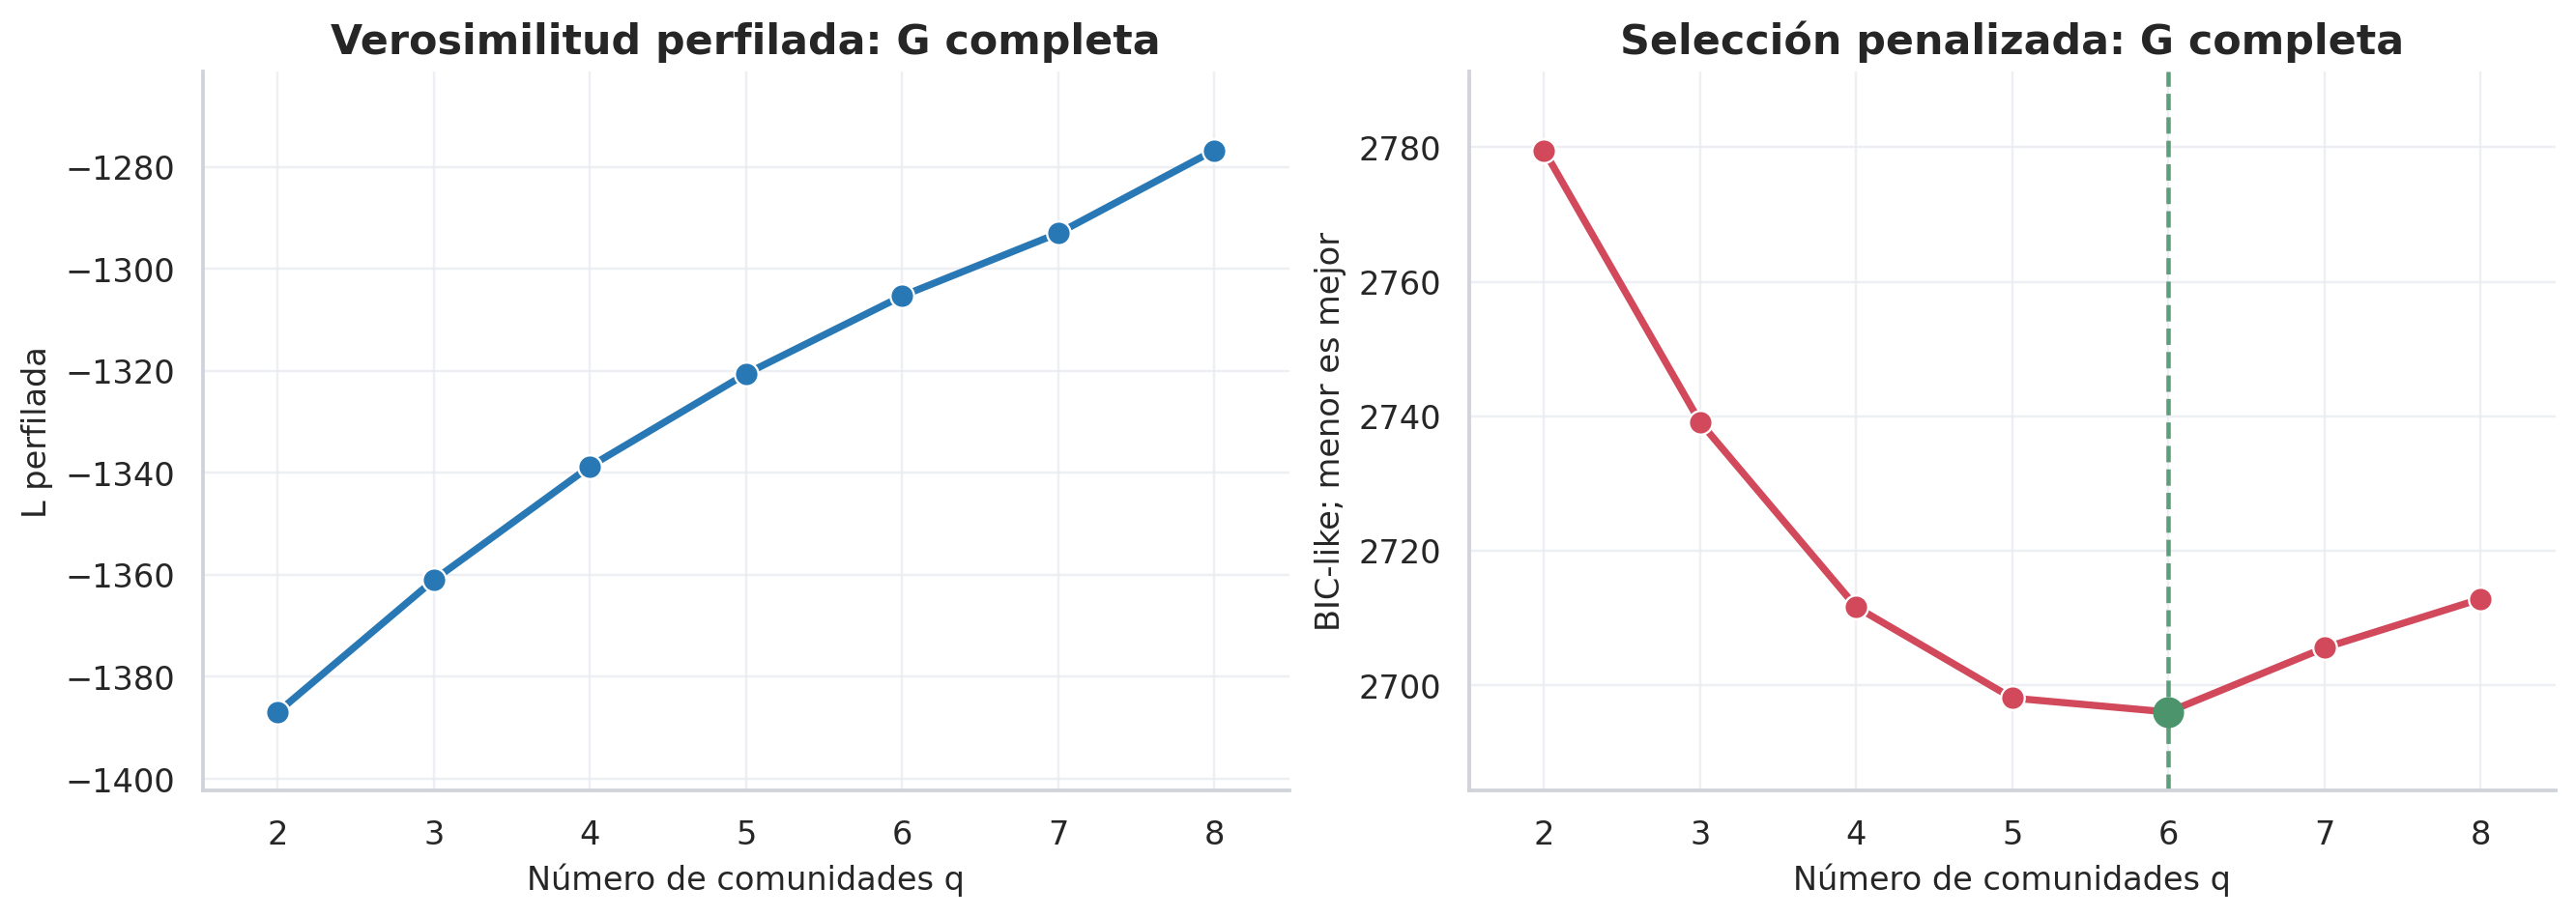
\includegraphics[width=0.82\linewidth]{barrido_q_G_completa.png}
\caption{Barrido de $q$ en la red completa. El BIC-like selecciona $q=6$.}
\end{figure}

\begin{figure}[H]
\centering

\includegraphics[width=0.82\linewidth]{barrido_q_G_mini.png}
\caption{Barrido de $q$ en la minired. Al retirar personajes periféricos, el criterio selecciona $q=5$.}
\end{figure}

\section{Resultados en la red completa}

La notebook etiqueta los grupos como $C0,\ldots,C5$. En esta sección usamos la notación matemática:
\[
C0\equiv 1,\quad
C1\equiv 2,\quad
C2\equiv 3,\quad
C3\equiv 4,\quad
C4\equiv 5,\quad
C5\equiv 6.
\]

\begin{table}[H]
\centering
\caption{Comunidades estimadas en la red completa.}
\resizebox{\textwidth}{!}{%
\begin{tabular}{clrrrp{8.3cm}}
\toprule
Grupo & Lectura narrativa & Nodos & Internas & $\kappa_r$ & Miembros\\
\midrule
1 & Padmé y conectores periféricos & 6 & 0 & 70 & DARTH SIDIOUS, ELAN, PADMÉ, SHMI, WATTO, ZAM WESSEL\\
2 & Tatooine/Naboo y separatistas periféricos & 13 & 12 & 73 & BERU, CLIEGG, JOBAL, NUTE GUNRAY, OWEN, POGGLE, QUEEN JAMILLIA, RUWEE, RYOO \& POOJA, SIO BIBBLE, SOLA, SUN RIT, THREEPIO\\
3 & Obi-Wan como puente de investigación & 2 & 0 & 59 & DOOKU, OBI-WAN\\
4 & Anakin y Count Dooku como eje de cruce & 2 & 1 & 69 & ANAKIN, COUNT DOOKU\\
5 & Kamino/Jango & 9 & 8 & 35 & BOBA FETT, DEXTER JETTSTER, HERMIONE BAGWA, JANGO, JANGO FETT, JOCASTA NU, LAMA SU, PK-4, TAUN WE\\
6 & Senado/Jedi/República & 15 & 41 & 158 & AMIDALA, BAIL ORGANA, CAPTAIN TYPHO, CHILDREN, DORME, JAR JAR, KI-ADI-MUNDI, MACE, MACE WINDU, MAS AMEDDA, ORN FREE TAA, PALPATINE, SENATOR ASK AAK, WINDU, YODA\\
\bottomrule
\end{tabular}
}
\end{table}

Las matrices agregadas fueron
\[
M=
\begin{pmatrix}
0&19&7&25&1&18\\
19&34&3&17&0&0\\
7&3&0&14&16&19\\
25&17&14&2&0&11\\
1&0&16&0&18&0\\
18&0&19&11&0&110
\end{pmatrix},
\]
\[
\Omhat=
\begin{pmatrix}
0&1.725&0.786&2.402&0.189&0.755\\
1.725&2.960&0.323&1.566&0&0\\
0.786&0.323&0&1.596&3.595&0.946\\
2.402&1.566&1.596&0.195&0&0.468\\
0.189&0&3.595&0&6.818&0\\
0.755&0&0.946&0.468&0&2.045
\end{pmatrix}.
\]

\subsection{Bloques asortativos}

El bloque más claramente asortativo es el grupo 5, asociado a Kamino/Jango. Tiene $m_{55}=18$ y $\kappa_5=35$. Como $m=148$, entonces $2m=296$, y
\[
\hat\omega_{55}
=\frac{296\cdot 18}{35^2}
=6.818.
\]
Este valor es el más alto de toda la red completa. Matemáticamente, significa que el subgrupo Kamino/Jango tiene muchas más conexiones internas de las esperadas dado su volumen de grado. Narrativamente, tiene sentido: Jango Fett, Boba Fett, Taun We, Lama Su y personajes asociados forman una subtrama muy localizada.

También hay estructura asortativa en el grupo 2:
\[
\hat\omega_{22}=2.960,
\]
y en el grupo 6:
\[
\hat\omega_{66}=2.045.
\]
El grupo 6 es grande y contiene la esfera Senado/Jedi/República. Su masa interna es alta, $m_{66}=110$, pero su $\omega$ no es tan extremo como el grupo 5 porque también tiene un volumen de grado enorme: $\kappa_6=158$.

\subsection{Bloques puente y estructura de roles}

El cruce fuera de diagonal más fuerte es entre los grupos 3 y 5:
\[
m_{35}=16,
\qquad
\hat\omega_{35}=3.595.
\]
Este vínculo está explicado principalmente por Obi-Wan y los personajes de Kamino/Jango. La interpretación es clara: la investigación de Obi-Wan conecta la trama principal con Kamino y Jango Fett. El modelo no necesita poner a Obi-Wan dentro del bloque de Kamino; lo separa como un rol puente porque su patrón de conexión excede lo esperable hacia ese bloque.

Otro cruce importante es entre los grupos 1 y 4:
\[
m_{14}=25,
\qquad
\hat\omega_{14}=2.402.
\]
Este patrón refleja el eje Padmé--Anakin. El grupo 1 tiene a Padmé y conectores periféricos, mientras que el grupo 4 contiene a Anakin y Count Dooku. El modelo detecta que esa relación entre bloques es más importante que la densidad interna del grupo 1, que de hecho tiene $m_{11}=0$.

\begin{figure}[H]
\centering
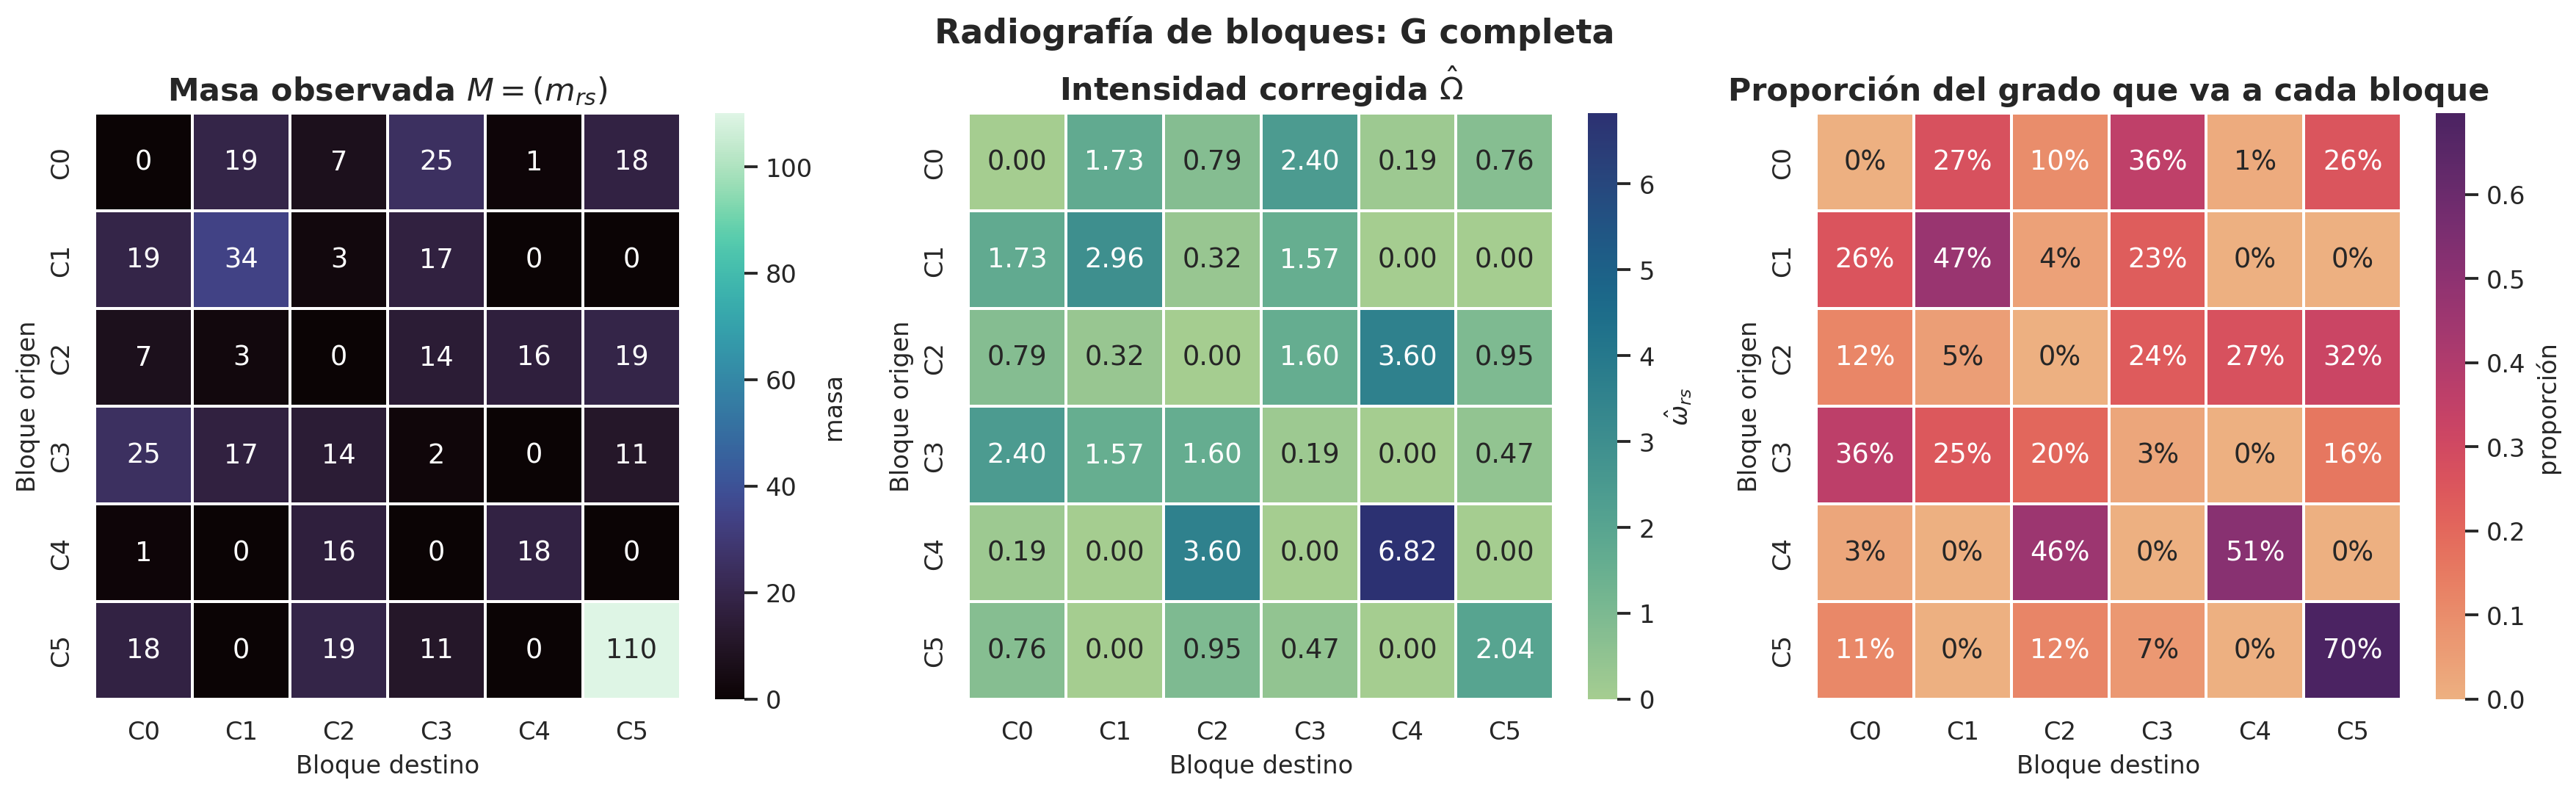
\includegraphics[width=0.96\linewidth]{radiografia_bloques_G_completa.png}
\caption{Radiografía de bloques para la red completa. Se observan diagonales fuertes en Kamino/Jango, Senado/Jedi y Tatooine/Naboo, además de cruces intensos entre roles narrativos.}
\end{figure}

\begin{figure}[H]
\centering
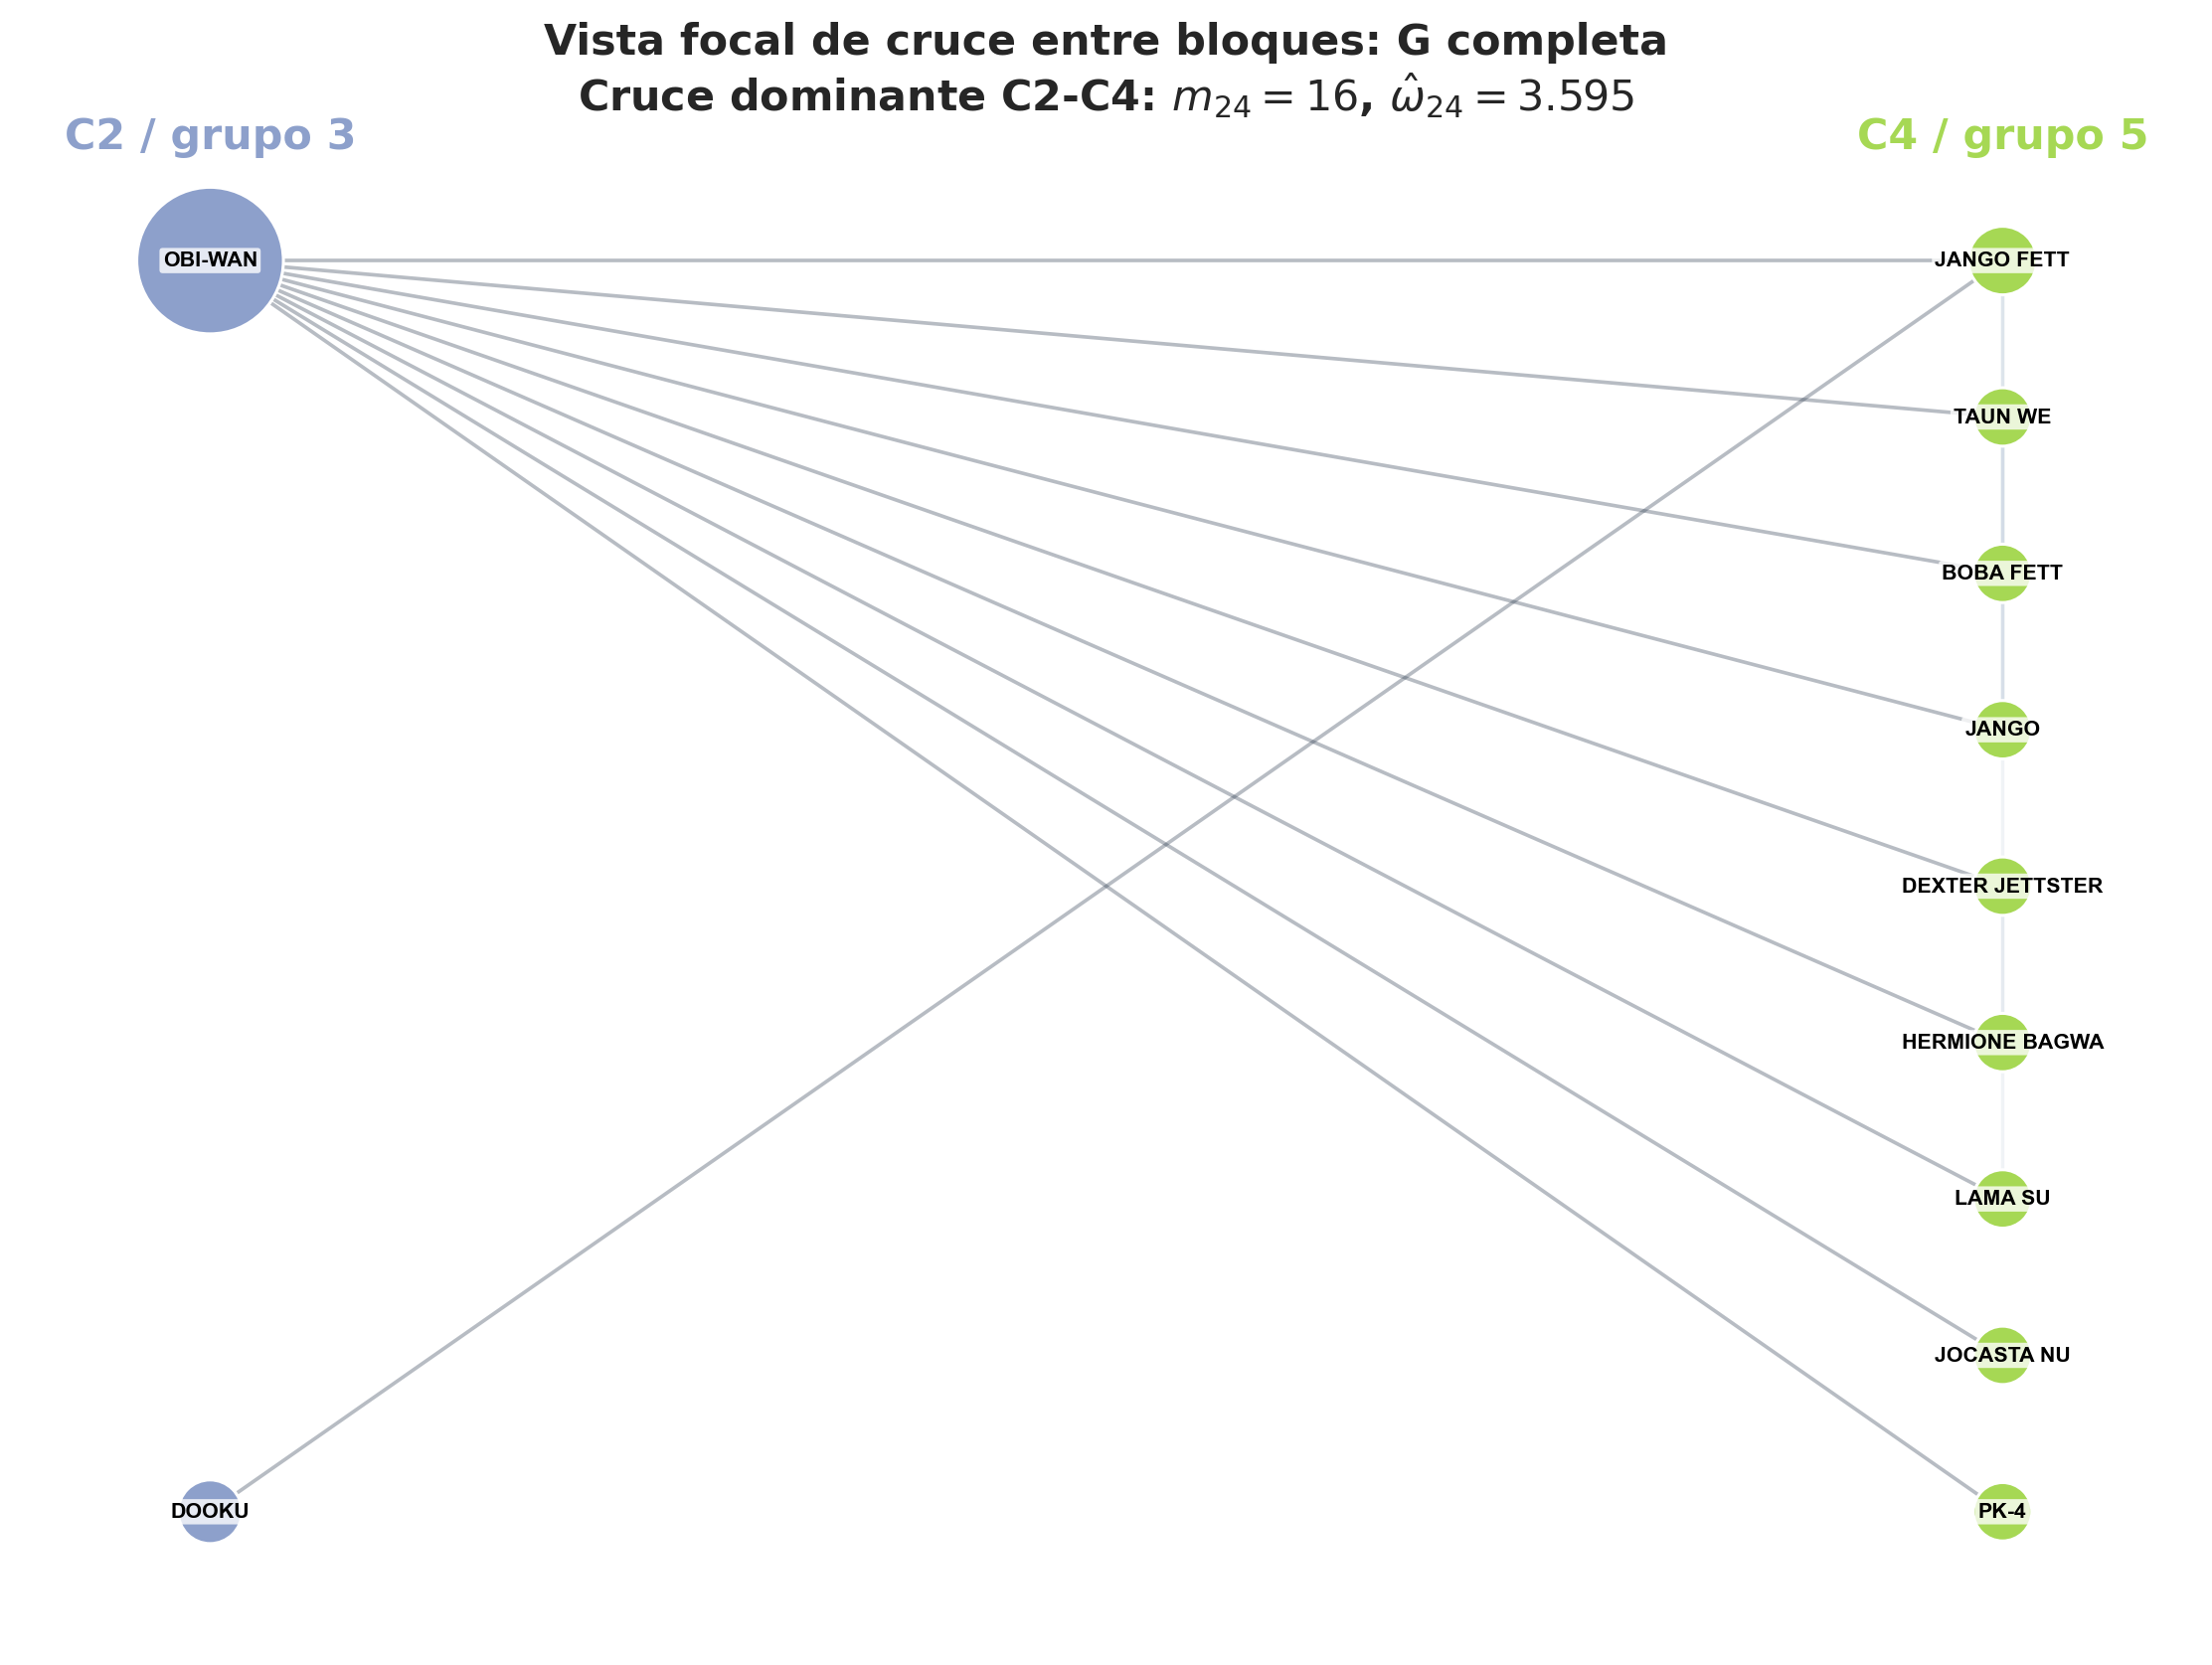
\includegraphics[width=0.86\linewidth]{vista_cruce_dominante_G_completa.png}
\caption{Vista focal del cruce dominante en la red completa: Obi-Wan y la subtrama Kamino/Jango.}
\end{figure}

\section{Resultados en la minired}

Al eliminar personajes de grado bajo, la minired selecciona $q=5$. La correspondencia es
\[
C0\equiv 1,\quad C1\equiv 2,\quad C2\equiv 3,\quad C3\equiv 4,\quad C4\equiv 5.
\]

\begin{table}[H]
\centering
\caption{Comunidades estimadas en la minired.}
\resizebox{\textwidth}{!}{%
\begin{tabular}{clrrrp{8.2cm}}
\toprule
Grupo & Lectura narrativa & Nodos & Internas & $\kappa_r$ & Miembros\\
\midrule
1 & Puentes centrales & 2 & 1 & 107 & OBI-WAN, PADMÉ\\
2 & Tatooine/Naboo y separatistas periféricos & 13 & 12 & 75 & BERU, CLIEGG, DORME, JOBAL, NUTE GUNRAY, OWEN, POGGLE, QUEEN JAMILLIA, RUWEE, SIO BIBBLE, SOLA, SUN RIT, THREEPIO\\
3 & Núcleo Kamino/Jango & 4 & 6 & 22 & BOBA FETT, JANGO, JANGO FETT, TAUN WE\\
4 & Senado/Jedi/República & 12 & 37 & 144 & AMIDALA, BAIL ORGANA, JAR JAR, KI-ADI-MUNDI, MACE, MACE WINDU, MAS AMEDDA, ORN FREE TAA, PALPATINE, SENATOR ASK AAK, WINDU, YODA\\
5 & Eje Anakin/Dooku/Typho & 3 & 2 & 70 & ANAKIN, CAPTAIN TYPHO, COUNT DOOKU\\
\bottomrule
\end{tabular}
}
\end{table}

Las matrices de la minired son
\[
M=
\begin{pmatrix}
8&23&8&31&37\\
23&34&0&0&18\\
8&0&14&0&0\\
31&0&0&102&11\\
37&18&0&11&4
\end{pmatrix},
\]
\[
\Omhat=
\begin{pmatrix}
0.292&1.198&1.421&0.841&2.065\\
1.198&2.527&0&0&1.433\\
1.421&0&12.091&0&0\\
0.841&0&0&2.056&0.456\\
2.065&1.433&0&0.456&0.341
\end{pmatrix}.
\]

El resultado se vuelve más nítido. El núcleo Kamino/Jango queda como un bloque pequeño y muy denso:
\[
\hat\omega_{33}
=12.091.
\]
Esto ocurre porque el bloque tiene $\kappa_3=22$ y $m_{33}=14$; la masa interna es enorme para un volumen de grado tan pequeño. En términos narrativos, al quitar personajes periféricos queda el subgrupo Jango/Boba/Taun We/Jango Fett como una escena o subtrama cerrada.

El cruce dominante en la minired es entre los grupos 1 y 5:
\[
m_{15}=37,
\qquad
\hat\omega_{15}=2.065.
\]
Los personajes que explican este cruce son Padmé, Obi-Wan, Anakin, Count Dooku y Captain Typho. Esto condensa el eje narrativo principal: la historia no separa limpiamente romance, investigación y conflicto político; los protagonistas conectan esas partes.

\begin{figure}[H]
\centering

\includegraphics[width=0.96\linewidth]{radiografia_bloques_G_mini.png}
\caption{Radiografía de bloques para la minired. El núcleo Kamino/Jango aparece con una diagonal extremadamente intensa.}
\end{figure}

\begin{figure}[H]
\centering
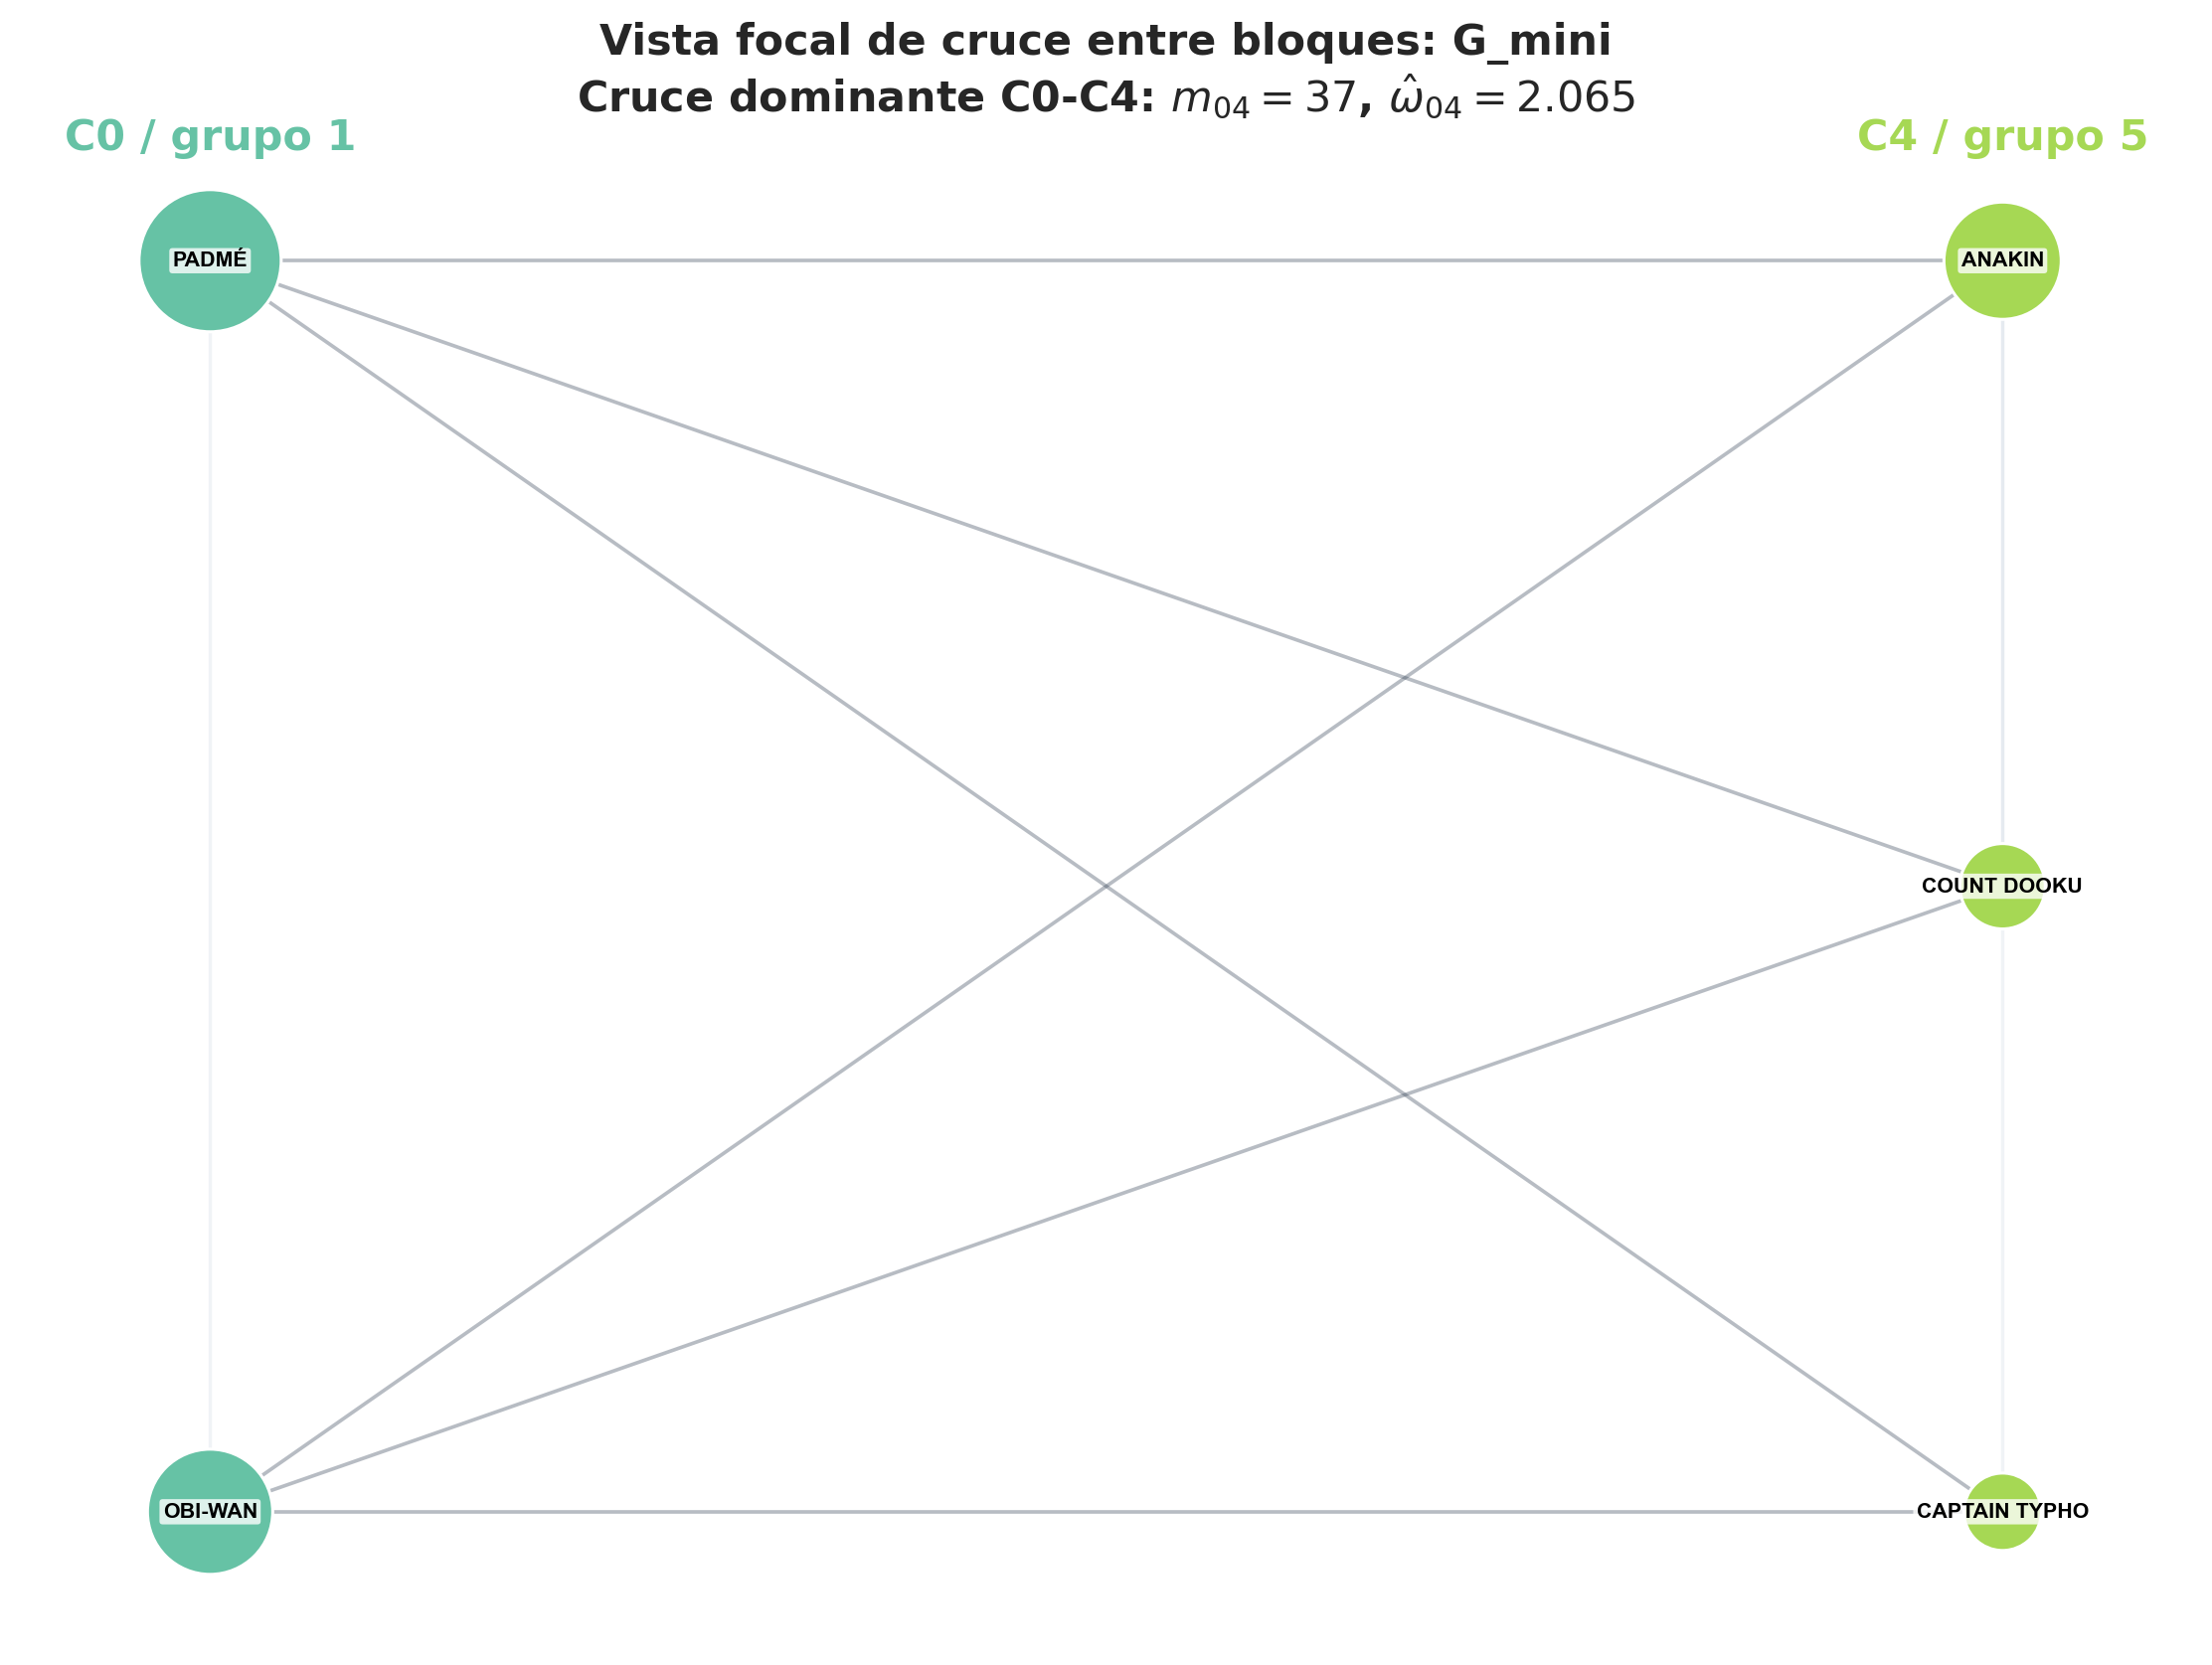
\includegraphics[width=0.86\linewidth]{vista_cruce_dominante_G_mini.png}
\caption{Vista focal del cruce dominante en la minired: los puentes centrales conectan con Anakin/Dooku/Typho.}
\end{figure}

\section{Lectura visual}

\begin{figure}[H]
\centering
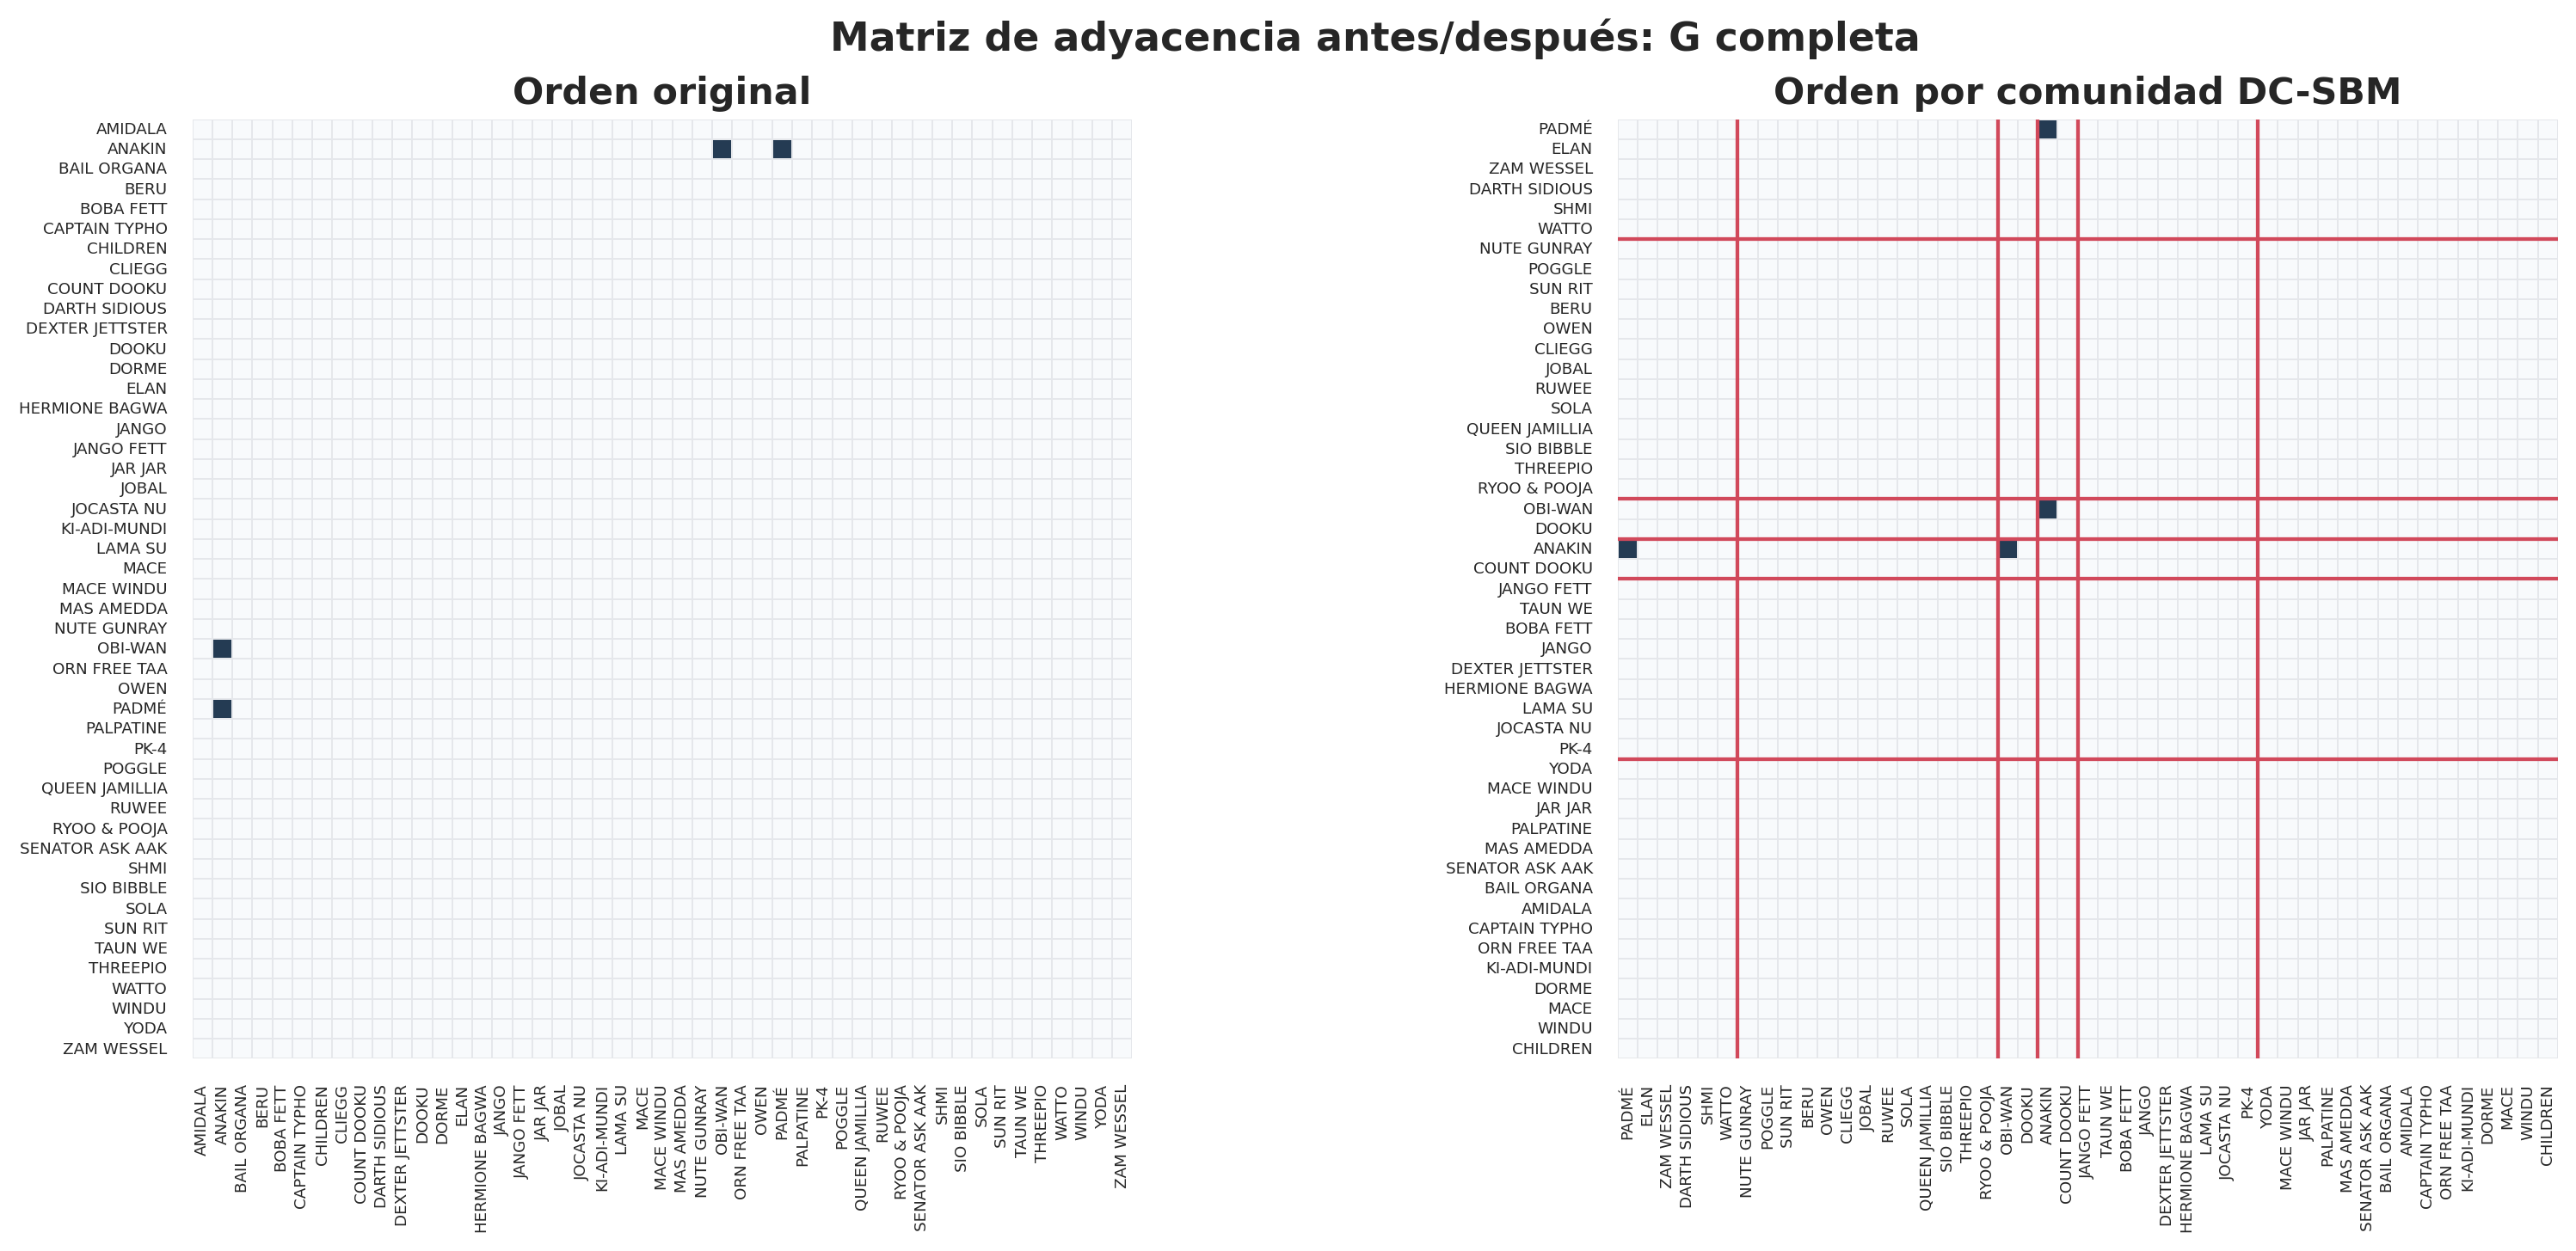
\includegraphics[width=0.95\linewidth]{adyacencia_antes_despues_G_completa.png}
\caption{Matriz de adyacencia de la red completa antes y después de ordenar por comunidades. El orden por DC-SBM revela bloques diagonales y cruces entre subtramas.}
\end{figure}

\begin{figure}[H]
\centering
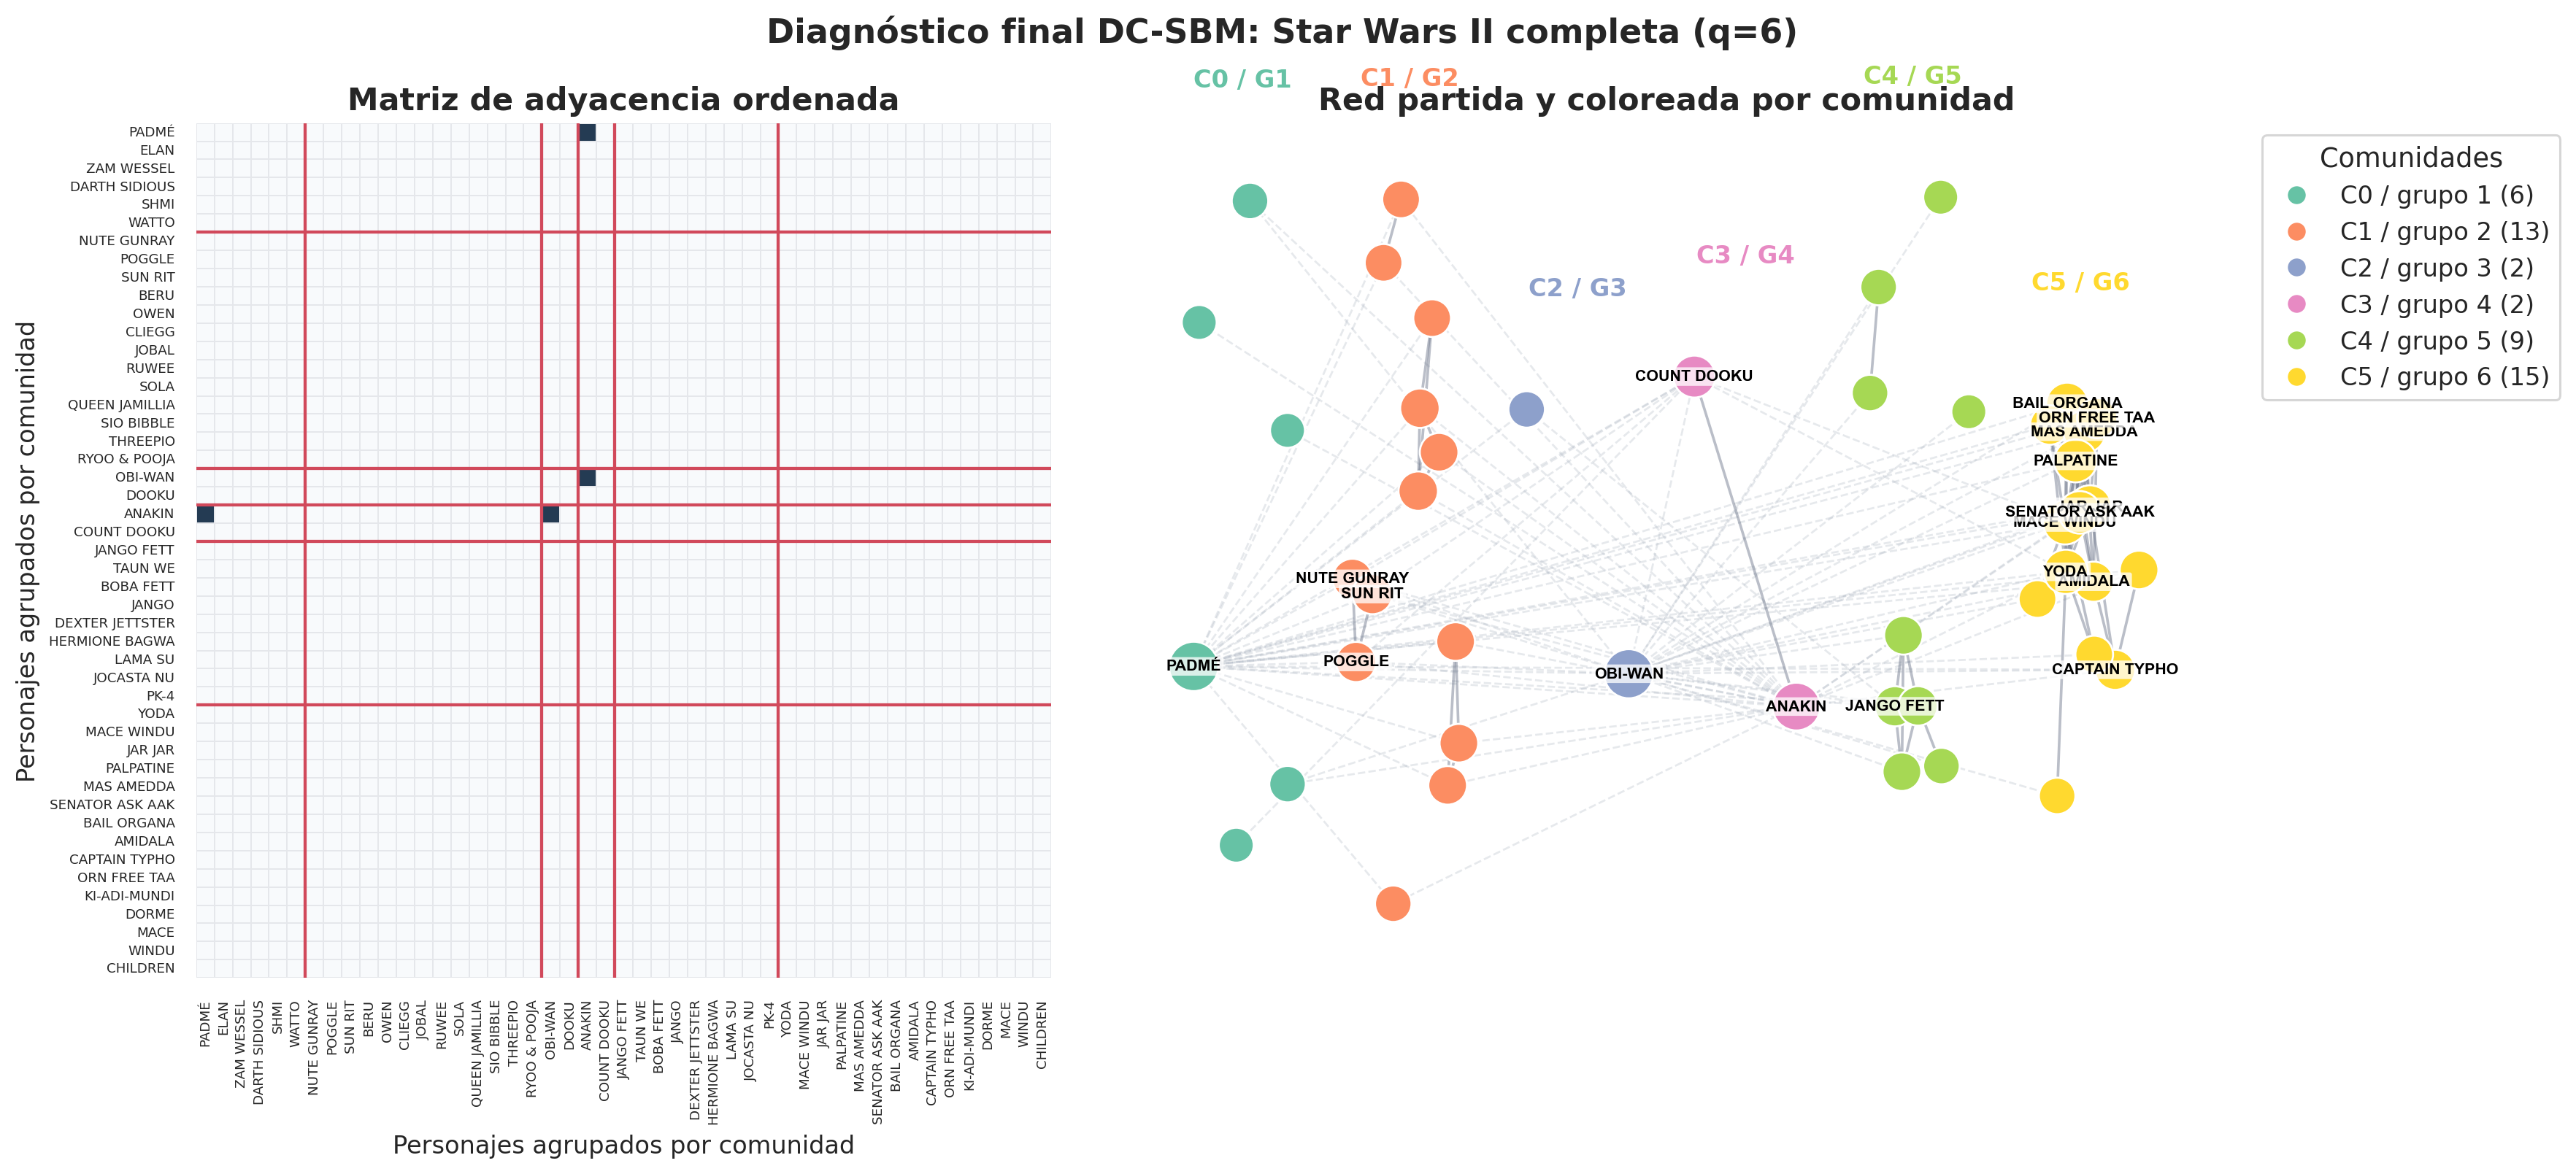
\includegraphics[width=0.95\linewidth]{final_adyacencia_y_red_partida_G.png}
\caption{Diagnóstico final de la red completa: matriz ordenada y red partida por comunidades.}
\end{figure}

Las figuras confirman tres hechos:
\begin{itemize}
    \item existen comunidades densas, como Kamino/Jango y Senado/Jedi;
    \item existen nodos puente, especialmente Padmé, Obi-Wan y Anakin;
    \item las comunidades no son puramente modulares, porque varias subtramas se explican mejor por cruces fuera de la diagonal.
\end{itemize}

\section{Explicación matemática de por qué pasa}

El modelo recompensa particiones que hacen grandes los términos
\[
m_{rs}\log\left(\frac{m_{rs}}{\kappa_r\kappa_s}\right).
\]
Por eso no basta con tener muchas aristas. Para que un par de bloques sea importante, la masa $m_{rs}$ debe ser grande relativa al producto $\kappa_r\kappa_s$.

En la red completa, el grupo 5 tiene $\kappa_5=35$ y $m_{55}=18$, por lo que
\[
\hat\omega_{55}=6.818.
\]
Aunque $18$ no es la masa más grande de toda la matriz, es enorme comparada con el volumen de grado del grupo. Por eso el DC-SBM lo considera un bloque muy concentrado.

En cambio, el grupo 6 tiene $m_{66}=110$, pero $\kappa_6=158$. Su intensidad es
\[
\hat\omega_{66}=2.045.
\]
Sigue siendo asortativa, pero no tan extrema, porque el grupo contiene muchos personajes de alto grado y por tanto se esperaría más conectividad interna aun bajo el modelo corregido por grado.

Los bloques puente se explican de forma análoga. El cruce grupos 3--5 tiene
\[
\hat\omega_{35}=3.595.
\]
Esto indica que la conexión Obi-Wan--Kamino/Jango es más intensa de lo esperable después de corregir por grado. El modelo separa a Obi-Wan como rol puente porque su patrón de aristas no es simplemente ``pertenecer'' al bloque Kamino: es conectar esa subtrama con el resto.

\section{Conclusión}

El resultado principal no es solamente que $q=6$ o $q=5$ sean buenos valores. La conclusión sustantiva es que la película tiene una red narrativa mixta:
\[
\boxed{
\text{subtramas densas}
\quad+\quad
\text{protagonistas puente}
\quad+\quad
\text{cruces entre roles narrativos}.
}
\]

El DC-SBM permite ver esta mezcla porque corrige por grado. Los personajes centrales no son agrupados solo por ser populares; el modelo pregunta si sus conexiones caen dentro de un bloque o entre bloques más de lo esperado. Así aparecen comunidades densas como Kamino/Jango, bloques institucionales como Senado/Jedi/República, y roles puente como Padmé, Obi-Wan y Anakin.

\end{document}
